\documentclass{homework}
% \usepackage{graphicx} % Required for inserting images
\usepackage{amsmath}
\usepackage{gensymb}
\usepackage{subfig}
\usepackage{float}

\class{ECEN 5427}
\title{Homework 1}
\author{Sean Jennings}
\date{February 20, 2025}

\begin{document}
\maketitle

\section{Problem 1}
\begin{enumerate}
    \item The first derivative is
    \begin{equation*}
        f'(x) = 2ax + b
    \end{equation*}
    and the second is
    \begin{equation*}
        f''(x) = 2a
    \end{equation*}

    \item
    \begin{letterenum}
    
    \item $f(x)$ is increasing when
    \begin{equation*}
         2ax + b = f'(x) > 0.
    \end{equation*}
    Subtracting $b$ and dividing by $2a$ gives
    \begin{equation*}
        x > \frac{-b}{2a}
        \label{eq:x-greater}
    \end{equation*}
    when $a > 0$ and 
    \begin{equation*}
        x < \frac{-b}{2a}
        \label{eq:x-less}
    \end{equation*}
    when $a < 0$ (since dividing by a negative flips the inequality sign).

    When $a = 0$, $f$ is a linear function and it is increasing if $b>0$.
    \item $f$ is decreasing under the opposite conditions as above. When
    \begin{enumerate}
        \item $a<0$ and $x > \frac{-b}{2a}$,
        \item $a>0$ and $x < \frac{-b}{2a}$, or
        \item $a=0$ and $b<0$.
    \end{enumerate}
\end{letterenum}

\item If $a = 0$, the function is linear, $f(x) = bx + c$, and the situation
is similar to part 2. $f(x) \geq 0$ when any of the following conditions hold:
\begin{letterenum}
    \item $b > 0$ and $x \geq -b/c$, or
    \item $b < 0$ and $x \leq -b/c$, or
    \item $b = 0$ and $c > 0$.
\end{letterenum}

When $a \neq 0$, the equation is quadratic, so the zeros are given by:
\begin{equation*}
    x_{1,2} = \frac{-b \pm \sqrt{b^2 - 4ac}}{2a}
\end{equation*}
There are three cases depending on the value of the discriminant.

First, if $b^2 - 4ac > 0$, there are two distinct zeros $x_1 < x_2$. If the
quadratic is convex (i.e. $a>0$), then $f(x)\geq0$ outside of the zeros,
$x \leq x_1$ or $x \geq x_2$. If it is concave ($a<0$), then $f(x)$ is nonnegative
within the closed interval $x_1 \leq x \leq x_2$. 

Second, if $b^2 - 4ac < 0$, there are no zeros, so either $f(x) \geq 0$ for all $x$
(if $a > 0$) or for no values of $x$ (if $a < 0$).

Last, When the discriminant is exactly 0, $f(x)$ has exactly one zero. If the
function is convex, it is again positive for all $x$. If it is concave, $f(x) \geq 0$
only at the zero, $x = x_1 = x_2$.

\end{enumerate}

\section{Problem 2}
\begin{enumerate}
    \item The supply curve for the EMRB and EMDD market is shown in tables \ref{tab:EMRB-supply}
    and \ref{tab:EMDD-supply}, respectively. The total capacity is 242 MW in EMRB and 293 MW in EMDD.

    \begin{table}
        \centering
        \begin{tabular}{|c|c|c|c|}
            \hline
            Name & Price (\$/MWh) & Capacity (MW) & Cumulative (MW) \\
            \hline
            G3  &    0 &     32  &         32 \\
            G5  &   15 &     68  &        100 \\
            G2  &   20 &    102  &        202 \\
            G4  &   42 &     25  &        227 \\
            G1  &   75 &     15  &        242 \\
            \hline
        \end{tabular}
        \caption{Supply curve for EMRB in tabular format}
        \label{tab:EMRB-supply}
    \end{table}

    \begin{table}
        \centering
        \begin{tabular}{|c|c|c|c|}
            \hline
            Name & Price (\$/MWh) & Capacity (MW) & Cumulative (MW) \\
            \hline
            G9  &   0  &    50        &      50 \\
            G10 &  12  &    65        &     115 \\
            G7  &  17  &   120        &     235 \\
            G8  &  40  &    35        &     270 \\
            G6  &  75  &    23        &     293 \\
            \hline
        \end{tabular}
        \caption{Supply curve for EMRB in tabular format}
        \label{tab:EMDD-supply}
    \end{table}


    \item The data in these tables is plotted in figures \ref{fig:EMRB-supply}
    and \ref{fig:EMDD-supply}.     
    The market equilibrium is the intersection between supply and demand
    curves. 
    
    The price is set by G2 at 20 \$/MWh in EMRB.
    In EMDD, the demand forecast is exactly at the boundary between
    G7 and G8. Any incremental capacity needed will be provided by G8
    so it sets the price at 40 \$/MWh.

    \begin{center}
        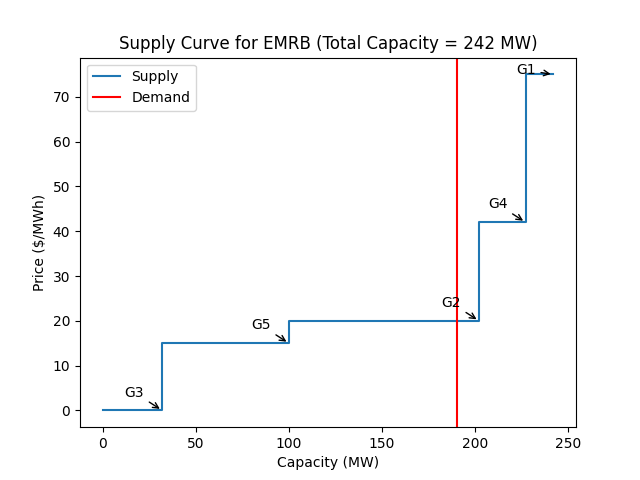
\includegraphics[width=0.8\linewidth]{Images/supply_EMRB.png}
        \captionof{figure}{EMRB Supply Curve --
        Note: the generator labels on the curve refer to the horizontal
            line which lies to the left of the arrow. All capacity along
            this horizontal line is supplied by the labeled generator.
        }
        \label{fig:EMRB-supply}
    \end{center}
    \begin{center}
        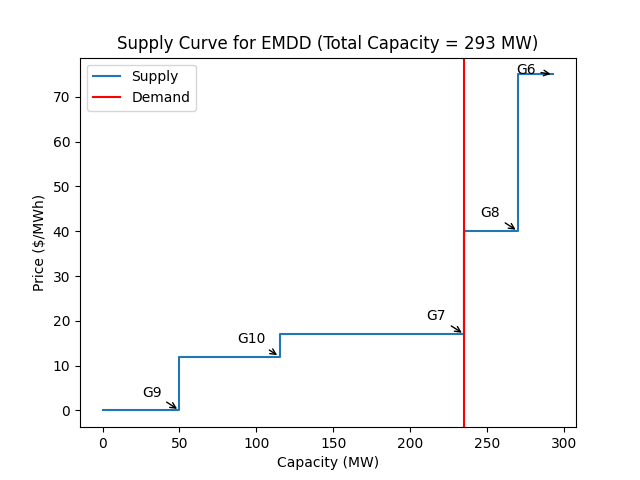
\includegraphics[width=0.8\linewidth]{Images/supply_EMDD.png}
        \captionof{figure}{EMDD Supply Curve}
        \label{fig:EMDD-supply}
    \end{center}

    \item The marginal generator in EMRB is G2, since any incremental capacity
    will be provided by this generator. As discussed in the previous part
    G8 is the marginal generator in EMDD. Any increases in demand will be met by G8.

    \item The generator set to "scheduled" to run will depend on the amount of operating reserve
    that is needed. Assuming that operating reserve and other ancilliary services are settled via a separate market,
    G3, G5, and G2 will be scheduled in EMRB, and G9, G10 and G7 will be scheduled in EMDD. The amount
    of energy provided by each generator is shown in tables \ref{tab:EMRB-rev} and \ref{tab:EMDD-rev}.
    
    Depending on the amount of operating reserves required, it's possible that G8 or G4 will also be
    required, but that will be settled closer to real-time when the demand forecast is more accurate.

    \begin{table}
        \centering
        \begin{tabular}{|c|c|c|c|}
            \hline
            Name & Energy Supplied (MWh) &  Revenue (\$) & Profit (\$) \\
            \hline
            G3  &    32 &     640  &         640 \\
            G5  &    68 &     1360  &        340 \\
            G2  &    90 &    1800  &        0 \\
            G4  &    0  &     0  &        0 \\
            G1  &    0  &     0  &        0 \\
            \hline
        \end{tabular}
        \caption{Revenue and profits for EMRB (Energy price 20\$/MWh)}
        \label{tab:EMRB-rev}
    \end{table}

    \begin{table}
        \centering
        \begin{tabular}{|c|c|c|c|}
            \hline
            Name & Energy Supplied (MWh) &  Revenue (\$) & Profit (\$) \\
            \hline
            G9   &     50 &     2000  &         2000 \\
            G10  &     65 &     2600  &        1820 \\
            G7   &    120 &    4800  &        2760 \\
            G8   &     0  &     0  &        0 \\
            G6   &     0  &     0  &        0 \\
            \hline
        \end{tabular}
        \caption{Revenue and profits for EMDD (Energy price 40\$/MWh)}
        \label{tab:EMDD-rev}
    \end{table}
    
    \item Revenue and profits are computed for EMRB and EMDD in tables \ref{tab:EMRB-rev} and \ref{tab:EMDD-rev},
    respectively.

    \item In EMRB, at 220 MWh, the G4 must also run, so price will increase from 20\$/MWh to 42\$ MWh. Since
    the price increases, all generators that were previously running will have increased revenue. Because
    G4 must also run in real-time, it's revenue will increase.

    In EMDD, at 250 MWh, the marginal price is still set by G8 and is therefore the same as in the day-ahead
    market. Since all the generators were scheduled at full capacity and the price is unchanged, all scheduled
    generators will make the same revenue. Since the difference between day-ahead and real-time demand is 
    met entirely by G8, it's revenues will increase because it is supplying more energy than purchased 
    in the day-ahead.


    \item G3 and G9 likely represent some form of renewable generation since they bid into the market at 0\$/MWh.
    This bid implies that the marginal cost of generation is zero. Renewables (like wind, solar, or geothermal)
    do not have any fuel costs and as a result do not have any marginal cost.

\end{enumerate}

\section{Problem 3}

\begin{enumerate}
    \item The tabulated representation of the demand curve for each market is shown 
    in tables \ref{tab:EMRB-dem} and \ref{tab:EMDD-dem}.
    Total demand is 224 MWh for EMRB and is 271 MWh and for EMDD.

\begin{table}
    \centering
    \begin{tabular}{|c|c|c|c|}
        \hline
        Name & Price (\$/MWh) & Demand (MWh) &   Cumulative Demand (MWh) \\
        \hline
        D2  &     78   &     23   &   23  \\
        D1  &     65   &     35   &   58  \\
        D5  &     64   &     43   &  101  \\
        D7  &     50   &     56   &  157  \\
        D4  &     46   &     38   &  195  \\
        D6  &     32   &     17   &  212  \\
        D3  &     10   &     12   &  224  \\
        \hline
    \end{tabular}
    \caption{Cumulative demand data for EMRB}
    \label{tab:EMRB-dem}
\end{table}

\begin{table}
    \centering
    \begin{tabular}{|c|c|c|c|}
        \hline
        Name & Price (\$/MWh) & Demand (MWh) &   Cumulative Demand (MWh) \\
        \hline
            D9       & 80     &          62    &         62 \\
            D8       & 72     &          48    &        110 \\
            D12      & 64     &          48    &        158 \\
            D14      & 48     &          30    &        188 \\
            D11      & 42     &          50    &        238 \\
            D13      & 32     &          18    &        256 \\
            D10      & 10     &          15    &        271 \\
        \hline
    \end{tabular}
    \caption{Cumulative demand data for EMDD}
    \label{tab:EMDD-dem}
\end{table}

    \item A plot of supply and demand curves are shown in figures \ref{fig:EMRB-demand}
    and \ref{fig:EMDD-demand}.
    
    The market equilibrium point for EMRB is where the D6
    portion of the demand curve intersects the vertical line between G2 and G4 sections
    of the supply curve. Thus, the market price is set by D6 at 32\$/MWh.
    The total energy supplied is cumulative capacity when all generators at and below
    G2 on the dispatch stack are running. From table \ref{tab:EMRB-supply}, this
    is 202 MWh.

    For EMDD, the curves intersect at G8 and the vertical line on the demand curve
    between D11 and D13. So the price is set by G8 at 40\$/MWh and the energy
    by the cumulative up to (and including) D11, i.e. 238 MWh.

    \begin{center}
        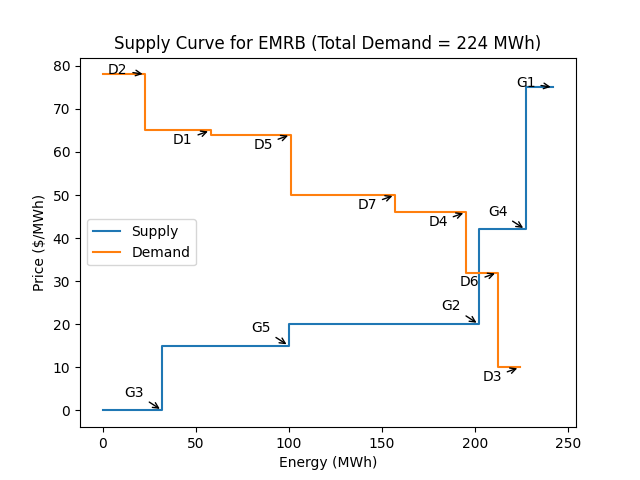
\includegraphics[width=0.8\linewidth]{Images/demand_EMRB.png}
        \captionof{figure}{EMRB Supply-Demand Curve --
        Note: as with supply curves in the previous figures, the demand labels refer to the horizontal
            line which lies to the left of the arrow. All demand along
            this horizontal line is demanded by the labeled load.
        }
        \label{fig:EMRB-demand}
    \end{center}
    \begin{center}
        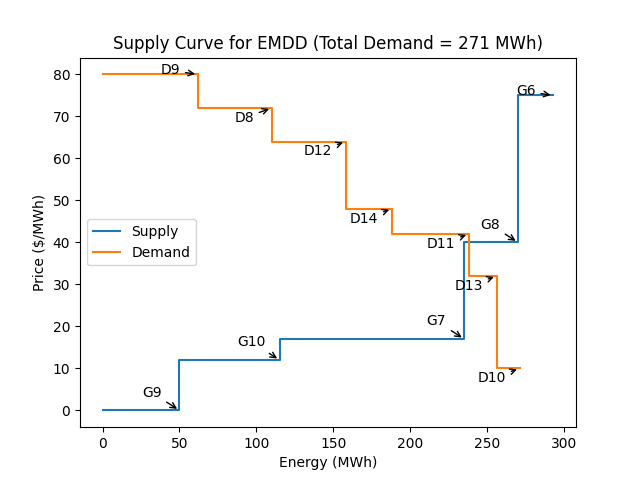
\includegraphics[width=0.8\linewidth]{Images/demand_EMDD.png}
        \captionof{figure}{EMDD Supply-Demand Curve}
        \label{fig:EMDD-demand}
    \end{center}


    \item The marginal generator is G4 in the EMRB market, since it will supply additional demand
        (when the demand is bid above the marginal cost of G4's generation). However, it is the
        demand D6 which sets the price. Therefore, D6 is the marginal unit in the sense that
        any change in the bid price will change the market clearing price.

        In EMDD, the marginal generator is G8 since it's bid sets the market price. D11 is the marginal
        demand in the sense that any increase in the quantity of energy demanded by this load will affect
        the amount that is generated by G8 (although without changing the price!).


    \item The energy generated by each each producer in the EMRB and EMDD markets
    are shown in tables \ref{tab:EMRB-dem-rev} and \ref{tab:EMDD-dem-rev}, respectively.
    We see G3, G5, and G2 are running in EMRB and G9, G10, G7, and G8 in EMDD.

    The energy drawn by each consumer for the EMRB and EMDD markets are shown in tables
    \ref{tab:EMRB-costs} and \ref{tab:EMDD-costs}.
    
    \item The revenue, profits of each generator and the total costs of consumption are tabulated alongside
    the results of previous question.

\begin{table}
    \centering
    \begin{tabular}{|c|c|c|c|}
        \hline
        Name & Energy Generated (MWh) & Revenue (\$) &  Profit (\$) \\
        \hline
        G3  &    32 &      1024  &       1024 \\
        G5  &    68 &      2176  &       1156 \\
        G2  &   102 &      3264  &       1224 \\
        G4  &     0 &         0  &          0 \\
        G1  &     0 &         0  &          0 \\
        \hline
    \end{tabular}
    \caption{Generation, Revenue, and Profit in EMRB market}
    \label{tab:EMRB-dem-rev}
\end{table}

\begin{table}
    \centering
    \begin{tabular}{|c|c|c|c|}
        \hline
        Name & Energy Generated (MWh) & Revenue (\$) &  Profit (\$) \\
        \hline
        G9  &    50 &      2000  &       2000 \\
        G10 &    65 &      2600  &       1820 \\
        G7  &   120 &      4800  &       2760 \\
        G8  &     3 &       120  &          0 \\
        G6  &     0 &         0  &          0 \\
        \hline
    \end{tabular}
    \caption{Generation, Revenue, and Profit in EMDD market}
    \label{tab:EMDD-dem-rev}
\end{table}

\begin{table}
    \centering
    \begin{tabular}{|c|c|c|c|}
        \hline
        Name & Energy Consumed (MWh) & Total Cost (\$)  \\
        \hline
            D2   &   23 &         736 \\
            D1   &   35 &        1120 \\
            D5   &   43 &        1376 \\
            D7   &   56 &        1792 \\
            D4   &   38 &        1216 \\
            D6   &    7 &         224 \\
            D3   &    0 &           0 \\
        \hline
    \end{tabular}
    \caption{Consumption and costs in EMRB}
    \label{tab:EMRB-costs}
\end{table}

\begin{table}
    \centering
    \begin{tabular}{|c|c|c|c|}
        \hline
        Name & Energy Consumed (MWh) & Total Cost (\$)  \\
        \hline
        D9    &  62  &       2480 \\
        D8    &  48  &       1920 \\
        D12   &  48  &       1920 \\
        D14   &  30  &       1200 \\
        D11   &  50  &       2000 \\
        D13   &   0  &          0 \\
        D10   &   0  &          0 \\
        \hline
    \end{tabular}
    \caption{Consumption and costs in EMDD}
    \label{tab:EMDD-costs}
\end{table}


\item The supply-demand curve for the combined market is shown in Figure
\ref{fig:combined-market}. The market's equilibrium position
is at 437 MWh total energy generation/consumption at 32\$/MWh.

The amount of energy production is determined by the cumulative generation 
of all plants up to and including G2. The price is set
by the D6 and D13 demand bids.

The cost of electricity is the same in the combined market as it was in EMRB, 
but has reduced from the price in EMDD. This means that consumers and generators
previously the EMDD market spend and earn less, respectively, than if the markets
were separating. This benefits EMDD consumers and hurts EMDD generators. Of course,
this exercise only represents a 1 hr snapshot and in the long-run it is likely that 
both markets benefit, if only from improved reliability and distribution of risk.

\begin{center}
    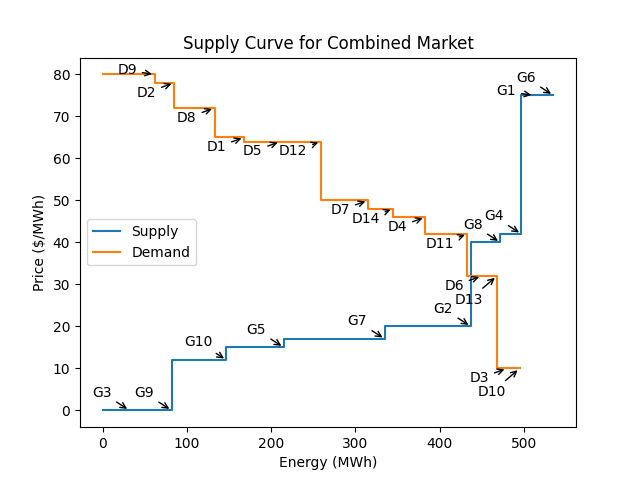
\includegraphics[width=0.8\linewidth]{Images/demand_total.png}
    \captionof{figure}{Supply-Demand Curve for combined market}
    \label{fig:combined-market}
\end{center}
\end{enumerate}


\end{document}
